%!TEX root = ../../thesis.tex

Relating raw detector output to physical particles in an incredibly difficult task,
particularly in a high pile-up environment. Sophisticated algorithms were developed for 
this task, and are outlined below.



\subsection{Tracks}
\label{sec:objects:tracks}

A track is a sequence of hits in the \ac{ID} indicative of a charged particle trajectory. 
To first approximation the trajectories are helical, owing to the pervading solenoidal 
magnetic field. However, multiple scattering and energy losses in the detector material 
and bremsstrahlung can cause significant deviations from this path. Track reconstruction 
is possible in the region $\mods{\eta} < 2.5$ (the extent of the \ac{ID}).

The inputs to the track reconstruction are threefold: pixel hits, \acs{SCT} 
space-points\footnote{
	Each SCT module comprises two layers of silicon strips with a small stereo angle, 
	enabling the three-dimensional position, or \textit{space-point}, to be precisely 
	measured (see \Section~\ref{sec:atlas:id}).
}
and \acs{TRT} drift circles. The \textit{inside-out} algorithm 
\cite{Tracking,ATLAS:ExpectPerf} uses a Kalman filter to seed tracks from hits in the 
three pixel layers and the first \acs{SCT} layer. The seeds are then extended and fitted 
into the \acs{SCT} and the \acs{TRT}, whilst resolving ambiguities and applying 
quality criteria. Finally, the \textit{outside-in} algorithm \cite{Tracking} considers 
unused track segments in the \acs{TRT}, and extrapolates them into the \acs{SCT} and 
pixel detector. This improves the tracking of secondary particles with a displaced vertex.



\subsection{Primary and secondary vertices}
\label{sec:objects:vertices}

A vertex is a location from which at least two outgoing tracks are reconstructed. 
\textit{Primary vertices} are associated with the interactions of incoming protons, 
whereas \textit{secondary vertices} are caused by particle decay or photon conversion
(\epluseminus pair production).

Primary vertex reconstruction has two steps: association of tracks to vertices 
(\textit{vertex finding}), and reconstruction of the vertex position itself 
(\textit{vertex fitting}). ATLAS employs an iterative \textit{finding-through-fitting} 
algorithm to simultaneously perform both steps \cite{PrimVertexFinding,AllVertexFinding}.
First, tracks originating from the interaction region 
(\unit{$\Delta z \approx 5.6$}{\centi\metre} and 
\unit{$\Delta r \approx 15$}{\micro\metre}) are identified and used to seed and fit a 
single vertex. Tracks considered outliers are then used to seed a new vertex, and a 
second fit of the two vertices is performed. The algorithm iterates, increasing the 
number of vertices, until the result stabilises.

The total number of primary vertices \npv is used to assess the pile-up conditions of 
the bunch crossing. The primary vertex of the hard scatter is chosen to be that with the 
highest $\sum p_{\text{T}}^2$ of the constituent tracks, and is referred to as simply \textit{the} 
primary vertex. As an additional quality criterion, this vertex must have at least three 
associated tracks.

Secondary vertex reconstruction is highly constrained by the physics of the vertex 
\cite{AllVertexFinding}. This can be enforced by mass or angular constraints, or in the 
track selection. For example, photon conversions are found using oppositely charged 
track pairs associated with electrons (via \acs{TRT} identification), with small 
opening angle. 
Flavour tagging of jets shall be described in \Section~\ref{sec:objects:bjets}.



\subsection{Electrons}
\label{sec:objects:electrons}

An electron will pass through the \ac{ID} before being absorbed by the \ac{ECal}. They 
are therefore reconstructed by matching a track with an energy cluster in the \ac{ECal}. 
Following reconstruction, the vast majority of electron objects are faked by hadrons, 
whilst many others are from photon conversions or electrons from heavy flavour decay (see 
\Figure~\ref{fig:objects:el_composition}). However, in the \HWWlvlv search, it is prompt 
electrons from the hard scatter that are of interest. Therefore identification and 
isolation criteria are applied to reject these backgrounds and select prompt electrons. 
The criteria were chosen to optimise the analysis sensitivity: \eg a low \et threshold 
of \unit{10}{\GeV} gives a large signal acceptance, but must be compensated by tight 
identification requirements to reject the large \Wjets and di-jet backgrounds.

Electrons with $\et > \unit{10}{\GeV}$ and $\mods{\eta} < 2.47$ are selected. Additionally, electrons with $1.37 < \mods{\eta} < 1.52$ are vetoed since they correspond
to the crack region (see \Section~\ref{sec:atlas:calo}).

\begin{figure}
	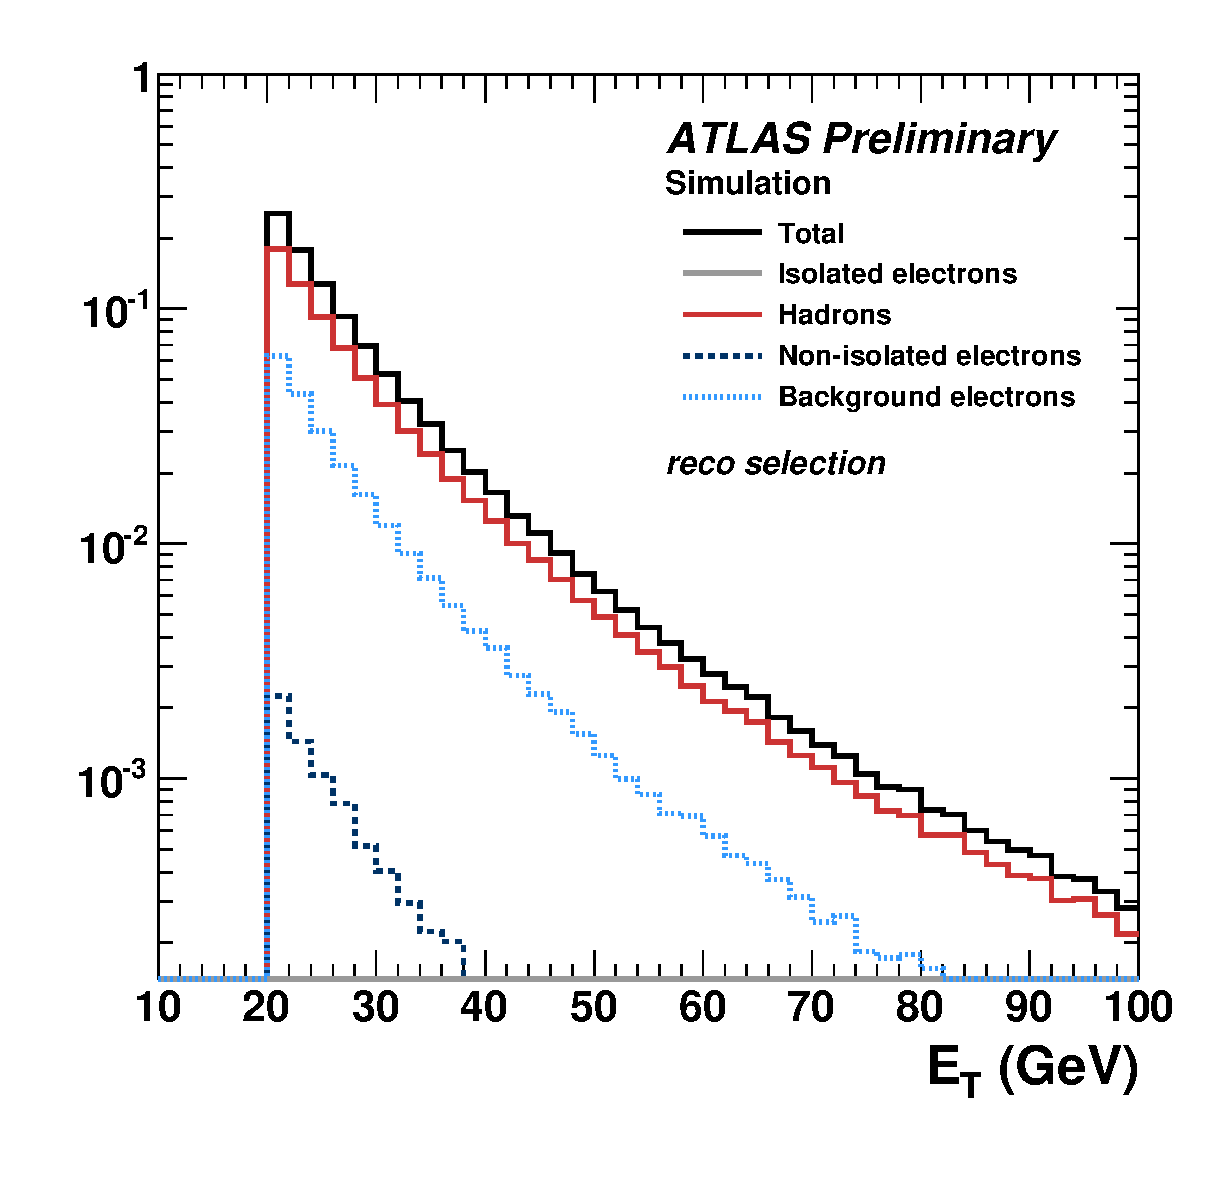
\includegraphics[width=\smallfigwidth]{tex/selection/electron_composition}
	\caption{The composition of reconstructed electrons as a function of transverse 
	energy, simulated by a \pythia{6} sample of di-jet, heavy flavour, prompt photon, \PW 
	and \PZ processes \cite{ElectronPerf:Expect}. Non-isolated electrons are from heavy 
	flavour decay. Background electrons are from photon conversions. Isolated electrons 
	are prompt electrons from a \PW or \PZ boson, though appear below the y-axis range.}
	\label{fig:objects:el_composition}
\end{figure}

\begin{description}
\item[Reconstruction] \hfill \\
	Energy deposits in \ac{ECal} cells are clustered by a \textit{sliding window} 
	algorithm \cite{ElectronPerf:Expect}. First, the calorimeter is divided into 
	\textit{towers} of size $\Delta\eta \times \Delta\phi = 0.025 \times 0.025$ (the 
	cell size of the middle layer). Then a window of $3 \times 5$ towers in $\eta$-$\phi$ 
	space scans the \ac{ECal} for local maxima with $\et > \unit{2.5}{\GeV}$.

	Tracks within $\Delta R < 0.3$ of a cluster are then refit using a Gaussian Sum 
	Filter (GSF) \cite{Electron:GSF}. The default fit described in 
	\Section~\ref{sec:objects:tracks} uses a pion hypothesis to estimate material 
	effects, and does not account for the significant bremsstrahlung experienced by 
	electrons (which is highly $\eta$-dependent). The GSF is a non-linear fitter and 
	improves the accuracy of electron tracking by accounting for this.

	For a cluster to be reconstructed as an electron, it must be matched to a track. If a 
	track is within $\Delta\eta < 0.05$ and $\Delta\phi < 0.1 (0.05)$ of the cluster 
	centre, they are considered matched. The asymmetric $\Delta\phi$ requirement allows 
	for increased bending due to bremsstrahlung. When multiple tracks are matched, that 
	with the smallest $\Delta R$ is chosen.

	Finally, the cluster is rebuilt using a $3 \times 7$ ($5 \times 5$) sliding window 
	in the barrel (end-cap), and the electron four-momentum is defined 
	\cite{ElectronPerf:2010}. The direction is taken from the matched track and the 
	energy is the cluster energy, corrected for losses in passive material and leakage 
	outside the cluster. These simulated corrections depend on the longitudinal shower 
	shape and energy deposited in the presampler. The EM energy scale was calibrated
	using test beam and \textit{in situ} \HepProcess{\PZ \HepTo \Pe\Pe} measurements.

\item[Identification] \hfill \\
	Electron identification is improved by applying cuts on track quality and shower 
	shape. There are three reference operating points called \textit{loose}, 
	\textit{medium} and \textit{tight}, with progressively greater background rejection 
	and lower signal efficiency.
	
	For $\et > \unit{25}{\GeV}$ the medium criteria are used, comprising cuts on
	\begin{itemize}[noitemsep,nolistsep]
		\item shower shape variables (lateral and longitudinal),
		\item leakage to the \ac{HCal},
		\item the number of pixel and \acs{SCT} hits,
		\item the impact parameter with respect to the primary vertex,
		\item track-cluster matching,
		\item transition radiation,
	\end{itemize}
	and additionally electrons with conversion vertices or without a hit in the first 
	pixel layer are vetoed (to suppress the \Wgamma background).
 
 	For $\et < \unit{25}{\GeV}$ the \Wjets and QCD backgrounds are much larger. Thus a 
 	multivariate \textit{very tight likelihood} identification is used, with similar 
 	signal efficiency to the cut-based tight criteria but improved background rejection. 
 	It uses the signal and background probability density functions of multiple input 
 	variables to construct a likelihood discriminant, which may be cut upon (effectively 
 	choosing an operating point). The input variables are similar to those used in 
 	medium identification, although track hits remain as cuts.

\item[Isolation] \hfill \\
	Rejection of hadronic fakes or electrons from heavy flavour decays is further 
	improved by requiring the electron to be isolated from activity in the tracker and 
	calorimeter. The cuts are summarised in \Table~\ref{tab:objects:el_iso} and explained 
	below.

	\begin{table}[b]
		\begin{tabular}{c@{\hskip 0.3in}c@{\hskip 0.3in}c}
			\toprule
			Electron \et (\GeV) & Tracker isolation & Calorimeter isolation \\
			\midrule
			10 -- 15 & $\ptcone{0.4}/\et < 0.06$ & $\etcone{0.3}/\et < 0.20$ \\
			15 -- 20 & $\ptcone{0.3}/\et < 0.08$ & $\etcone{0.3}/\et < 0.24$ \\
			$> 20$   & $\ptcone{0.3}/\et < 0.10$ & $\etcone{0.3}/\et < 0.28$ \\
			\bottomrule
		\end{tabular}
		\caption{Tracker and calorimeter isolation criteria for electrons. The cuts 
		were chosen to optimise the sensitivity of a low mass \HWWlvlv search.}
		\label{tab:objects:el_iso}
	\end{table}

	\textit{Tracker isolation:} $\ptcone{R_0}$ is the summed \pt of all tracks of 
	$\pt > \unit{0.4}{\GeV}$ within a cone of $\Delta R < R_0$, excluding the electron 
	track itself. For robustness against pile-up, the tracks are required to originate 
	from the primary vertex.

	\textit{Calorimeter isolation:} Uncalibrated topological clusters (see 
	\Section~\ref{sec:objects:jets}) are built from energy deposits in the \ac{ECal} 
	and \ac{HCal}. These are more robust against pile-up than cell deposits as they 
	suppress noise. $\etcone{R_0}$ is the summed \et of the topological clusters within a 
	cone of $\Delta R < R_0$, excluding cells in a $5 \times 7$ window around the 
	electron (see \Figure~\ref{fig:objects:el_iso}). Corrections are made for electron 
	energy leakage and deposits from pile-up and the underlying event.

	\begin{figure}
		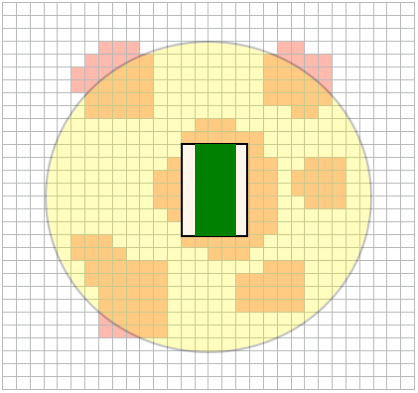
\includegraphics[width=0.8\smallfigwidth]{tex/selection/el_isolation}
		\caption{Schematic of calorimeter isolation. Pink cells constitute topological 
		clusters, the yellow circle is the isolation cone ($R_0 = 0.4$ shown), the green 
		$3 \times 7$ rectangle is the reconstructed electron cluster, and the white 
		$5 \times 7$ rectangle is the area removed from the cone.}
		\label{fig:objects:el_iso}
	\end{figure}

\item[Quality] \hfill \\
	An electron is rejected if its cluster is affected by a localised detector problem 
	(\eg a dead cell).

\item[Primary vertex association] \hfill \\
	To associate the electron with the primary vertex, the transverse impact parameter 
	$d_0$ is required to be within three standard deviations of zero. Also, the 
	longitudinal impact parameter $z_0$ is constrained by $\mods{z_0 \sin\theta} < 
	\unit{0.4}{\milli\metre}$.

\item[Efficiency] \hfill \\
	The efficiency of each selection step (reconstruction, identification, isolation and 
	primary vertex association) is measured via \textit{tag-and-probe} of 
	\HepProcess{\PZ \HepTo \Pe\Pe} events \cite{ElectronPerf:2010,ElectronPerf:2012}. 
	This involves selecting an unbiased sample of events containing a well-identified 
	\textit{tag} object and a loosely-identified \textit{probe} object, and measuring the 
	selection efficiency of the probes. The sample must be clean (often enforced by a 
	mass constraint) and backgrounds estimated (usually a side-bands or template fit).

	The tag is a well-identified electron, the probe is an electron passing the previous 
	step (or an \ac{ECal} cluster) and the constraint is $\unit{80}{\GeV} < 
	m_{\parenths{\text{tag, probe}}} < \unit{100}{\GeV}$. The reconstruction and 
	identification efficiencies are shown in \Figure~\ref{fig:objects:el_recoeff} and 
	\Figure~\ref{fig:objects:el_ideff} respectively. Comparison with MC yields efficiency 
	scale factors.

	\begin{figure}
		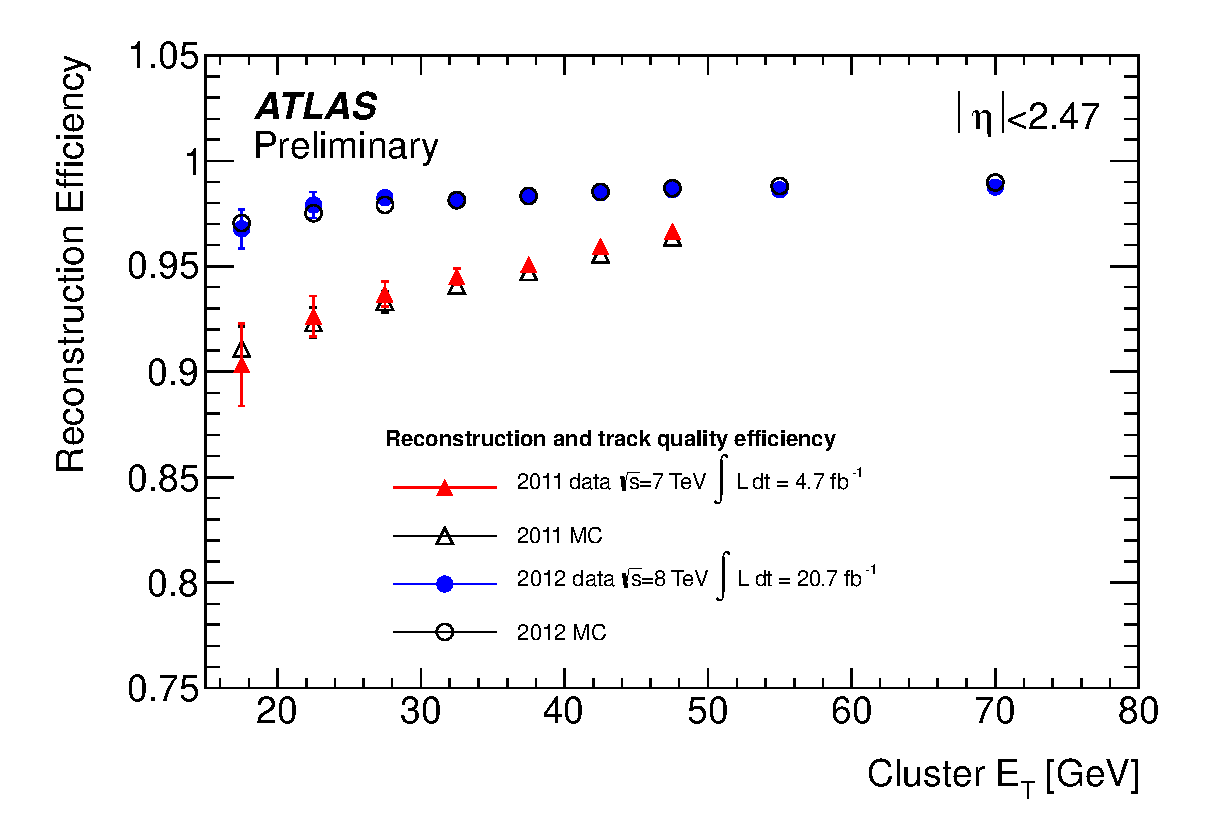
\includegraphics[width=0.495\textwidth]{tex/selection/el_recoeff_et}
		\hfill
		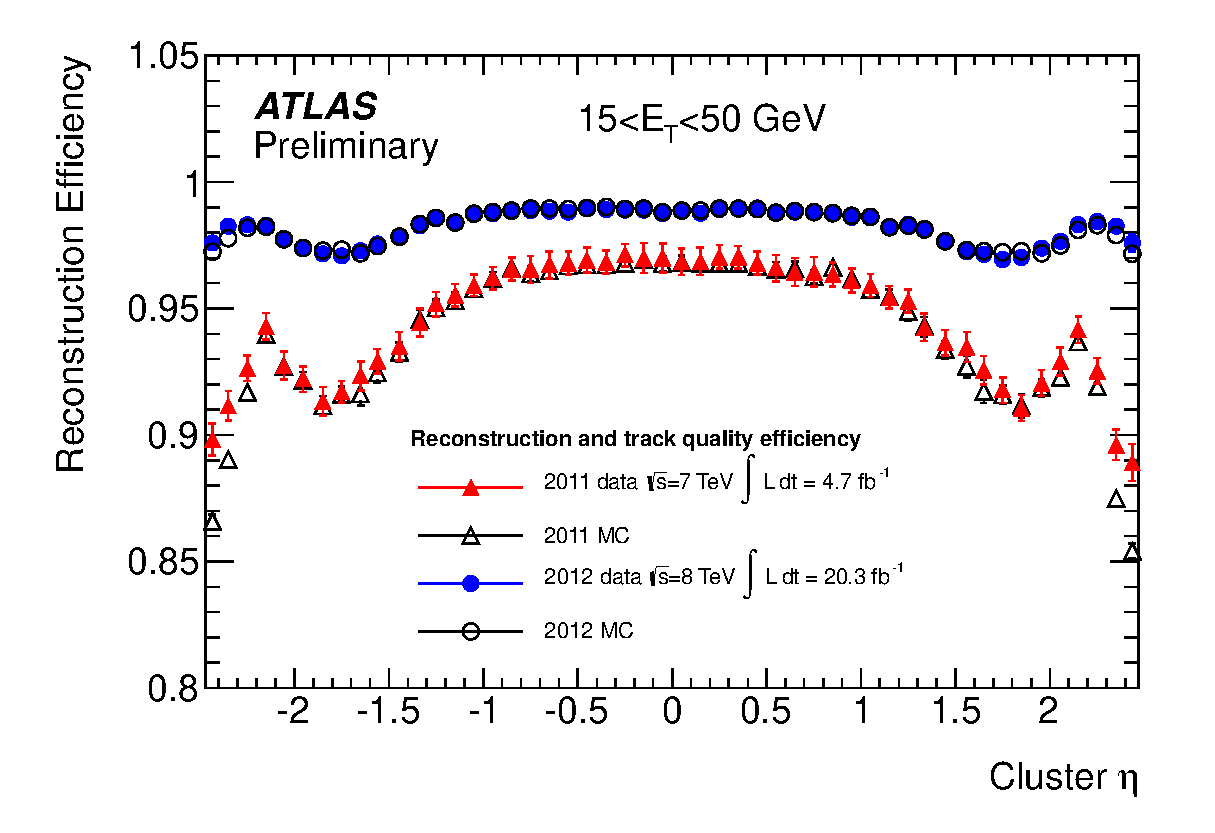
\includegraphics[width=0.495\textwidth]{tex/selection/el_recoeff_eta}
		\caption{Electron reconstruction efficiency versus \et (left) and $\eta$ (right), 
		measured using tag-and-probe of \HepProcess{\PZ \HepTo \Pe\Pe} data and compared 
		to MC \cite{ElectronPerf:2012}. In 2012, the implementation of GSF tracking gave 
		significant performance improvement.}
		\label{fig:objects:el_recoeff}
	\end{figure}

	\begin{figure}
		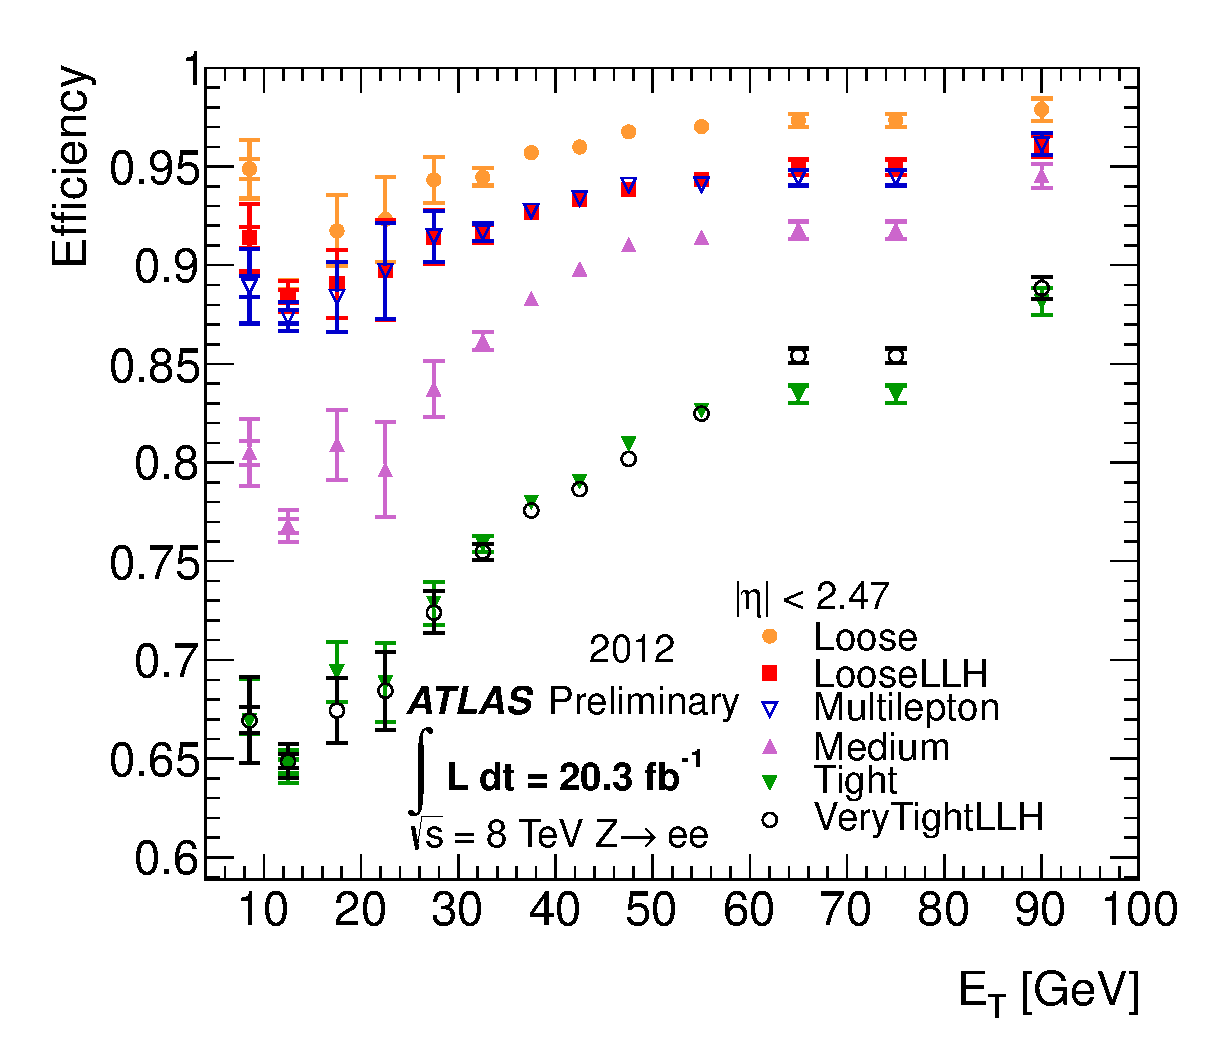
\includegraphics[width=0.495\textwidth]{tex/selection/el_ideff_et}
		\hfill
		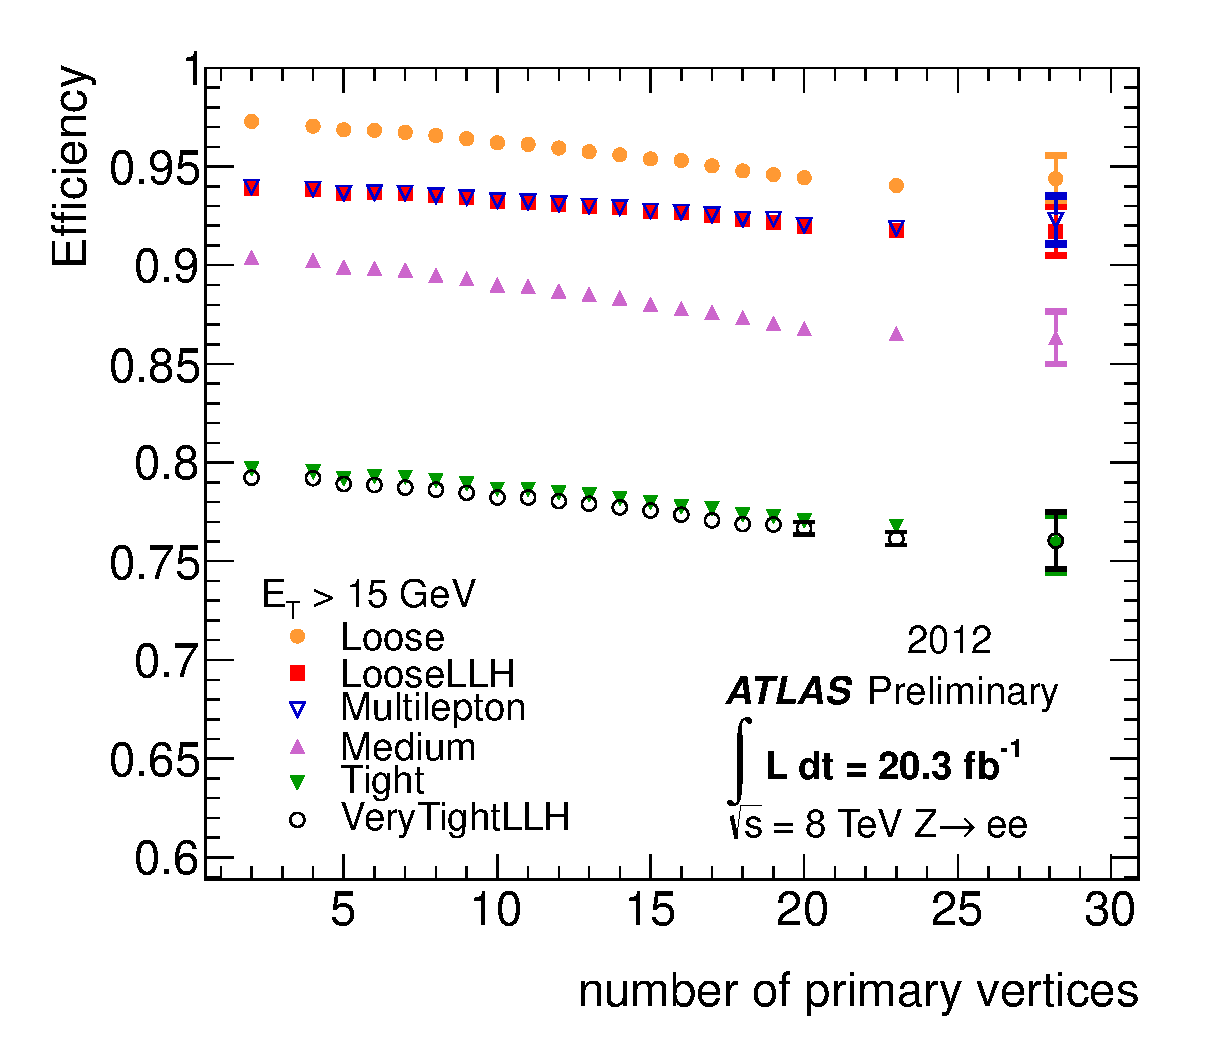
\includegraphics[width=0.495\textwidth]{tex/selection/el_ideff_npv}
		\caption{Efficiency of a variety of electron identification operating points 
		versus \et (left) and \npv (right), measured using tag-and-probe of 
		\HepProcess{\PZ \HepTo \Pe\Pe} data \cite{ElectronPerf:2012}. `Very tight 
		likelihood' has similar efficiency to `tight', but improves background rejection. 
		All operating points are fairly robust against pile-up.}
		\label{fig:objects:el_ideff}
	\end{figure}

\end{description}



\subsection{Muons}
\label{sec:objects:muons}

A muon will pass through the \ac{ID}, deposit minimal energy in the calorimeters and 
continue through the \ac{MS}. Thus, they can be found via activity in the \ac{MS}, 
optionally matched to an \ac{ID} track. Muons with $\pt > \unit{10}{\GeV}$ and 
$\mods{\eta} < 2.5$ are selected.

\begin{description}
\item[Reconstruction] \hfill \\
	Muons are found by matching \ac{MS} tracks to \ac{ID} tracks\footnote{
		A variety of muon reconstruction strategies are available: \textit{stand-alone} 
		muons have only \ac{MS} tracks, \textit{combined} muons have both \ac{MS} and 
		\ac{ID} tracks, \textit{segment-tagged} muons have \ac{ID} tracks that match to 
		\iac{MS} track segment, and \textit{calorimeter-tagged} muons have \ac{ID} 
		tracks matched to the calorimeter deposit of a minimum ionising particle (used to 
		recover efficiency at $\eta \approx 0$, where detector services reduce the \ac{MS}
		coverage). This thesis uses \textit{combined} muons, which perform best.
	}
	and their momenta are measured from track curvature \cite{ATLAS:ExpectPerf}.

	First, the \textit{Muonboy} algorithm \cite{Muons:algorithms} identifies a 
	$\Delta\eta \times \Delta\phi \approx 0.4 \times 0.4$ region of activity via the muon 
	trigger chambers (see \Section~\ref{sec:atlas:ms}) and then reconstructs localised 
	segments from nearby \acs{MDT} and \acs{CSC} hits. By scanning a potential momentum 
	range, segments in different layers are combined to form a track. Finally, a global 
	track fit using the full \ac{MS} hit information is performed, accounting for energy 
	loss.

	\ac{MS} tracks are extrapolated to the primary vertex, accounting for energy loss in 
	the calorimeter, and matched to \ac{ID} tracks (see 
	\Section~\ref{sec:objects:tracks}). The statistical combination of the two 
	tracks is performed by the \textit{STACO} algorithm \cite{Muons:algorithms}, which
	weights each track by its covariance matrix. The muon four-momentum is determined 
	from this combined track (dominated by the \ac{ID} track at low-\pt and by the 
	\ac{MS} track at high-\pt), and is calibrated with \HepProcess{\PZ \HepTo \Pmu\Pmu}
	events \cite{Muons:2012}.

\item[Isolation] \hfill \\
	Although the muon signature is much cleaner than that of electrons, hadronic fakes 
	(\textit{punch-through}) and muons from heavy flavour decays must still be suppressed 
	by isolation criteria, which are summarised in \Table~\ref{tab:objects:mu_iso}. The 
	$\ptcone{R_0}$ and $\etcone{R_0}$ variables are defined similarly to electrons, 
	though the size of the subtracted calorimeter window is reduced for muons.

	\begin{table}
		\begin{tabular}{c@{\hskip 0.3in}c@{\hskip 0.3in}c}
			\toprule
			Muon \pt (\GeV) & Tracker isolation & Calorimeter isolation \\
			\midrule
			10 -- 15 & $\ptcone{0.4}/\pt < 0.06$ & $\etcone{0.3}/\pt < 0.06$ \\
			15 -- 20 & $\ptcone{0.3}/\pt < 0.08$ & $\etcone{0.3}/\pt < 0.12$ \\
			20 -- 25 & $\ptcone{0.3}/\pt < 0.12$ & $\etcone{0.3}/\pt < 0.18$ \\
			$> 25$   & $\ptcone{0.3}/\pt < 0.12$ & $\etcone{0.3}/\pt < 0.30$ \\
			\bottomrule
		\end{tabular}
		\caption{Tracker and calorimeter isolation criteria for muons. The cuts were 
		chosen to optimise the sensitivity of a low mass \HWWlvlv search.}
		\label{tab:objects:mu_iso}
	\end{table}

\item[Quality] \hfill \\
	The \ac{ID} track must satisfy quality criteria on the number of traversed sensors:
	\begin{itemize}[noitemsep,nolistsep]
		\item $n_{\text{pixel}}^{\text{hit}} + n_{\text{pixel}}^{\text{dead}} \geq 1$
		\item $n_{\text{SCT}}^{\text{hit}} + n_{\text{SCT}}^{\text{dead}} \geq 5$
		\item $n_{\text{pixel}}^{\text{hole}} + n_{\text{SCT}}^{\text{hole}} \leq 2$
		\item $n_{\text{TRT}}^{\text{hit}} + n_{\text{TRT}}^{\text{outlier}} \geq 6$ and 
		at least 10\% are hits (for $\mods{\eta} < 1.9$ only)
	\end{itemize}
	where a hole is an expected hit that is not observed.

\item[Primary vertex association] \hfill \\
	To associate the muon with the primary vertex, the transverse impact parameter $d_0$ 
	is required to be within three standard deviations of zero. Also, the longitudinal 
	impact parameter $z_0$ is constrained by $\mods{z_0 \sin\theta} < 
	\unit{1.0}{\milli\metre}$.

\item[Efficiency] \hfill \\
	The efficiency of each selection step is measured via tag-and-probe of 
	\HepProcess{\PZ \HepTo \Pmu\Pmu} events \cite{Muons:2012}. For example, the 
	reconstruction efficiency is shown in \Figure~\ref{fig:objects:mu_recoeff}. 
	Comparison with MC yields efficiency scale factors.

	\begin{figure}
		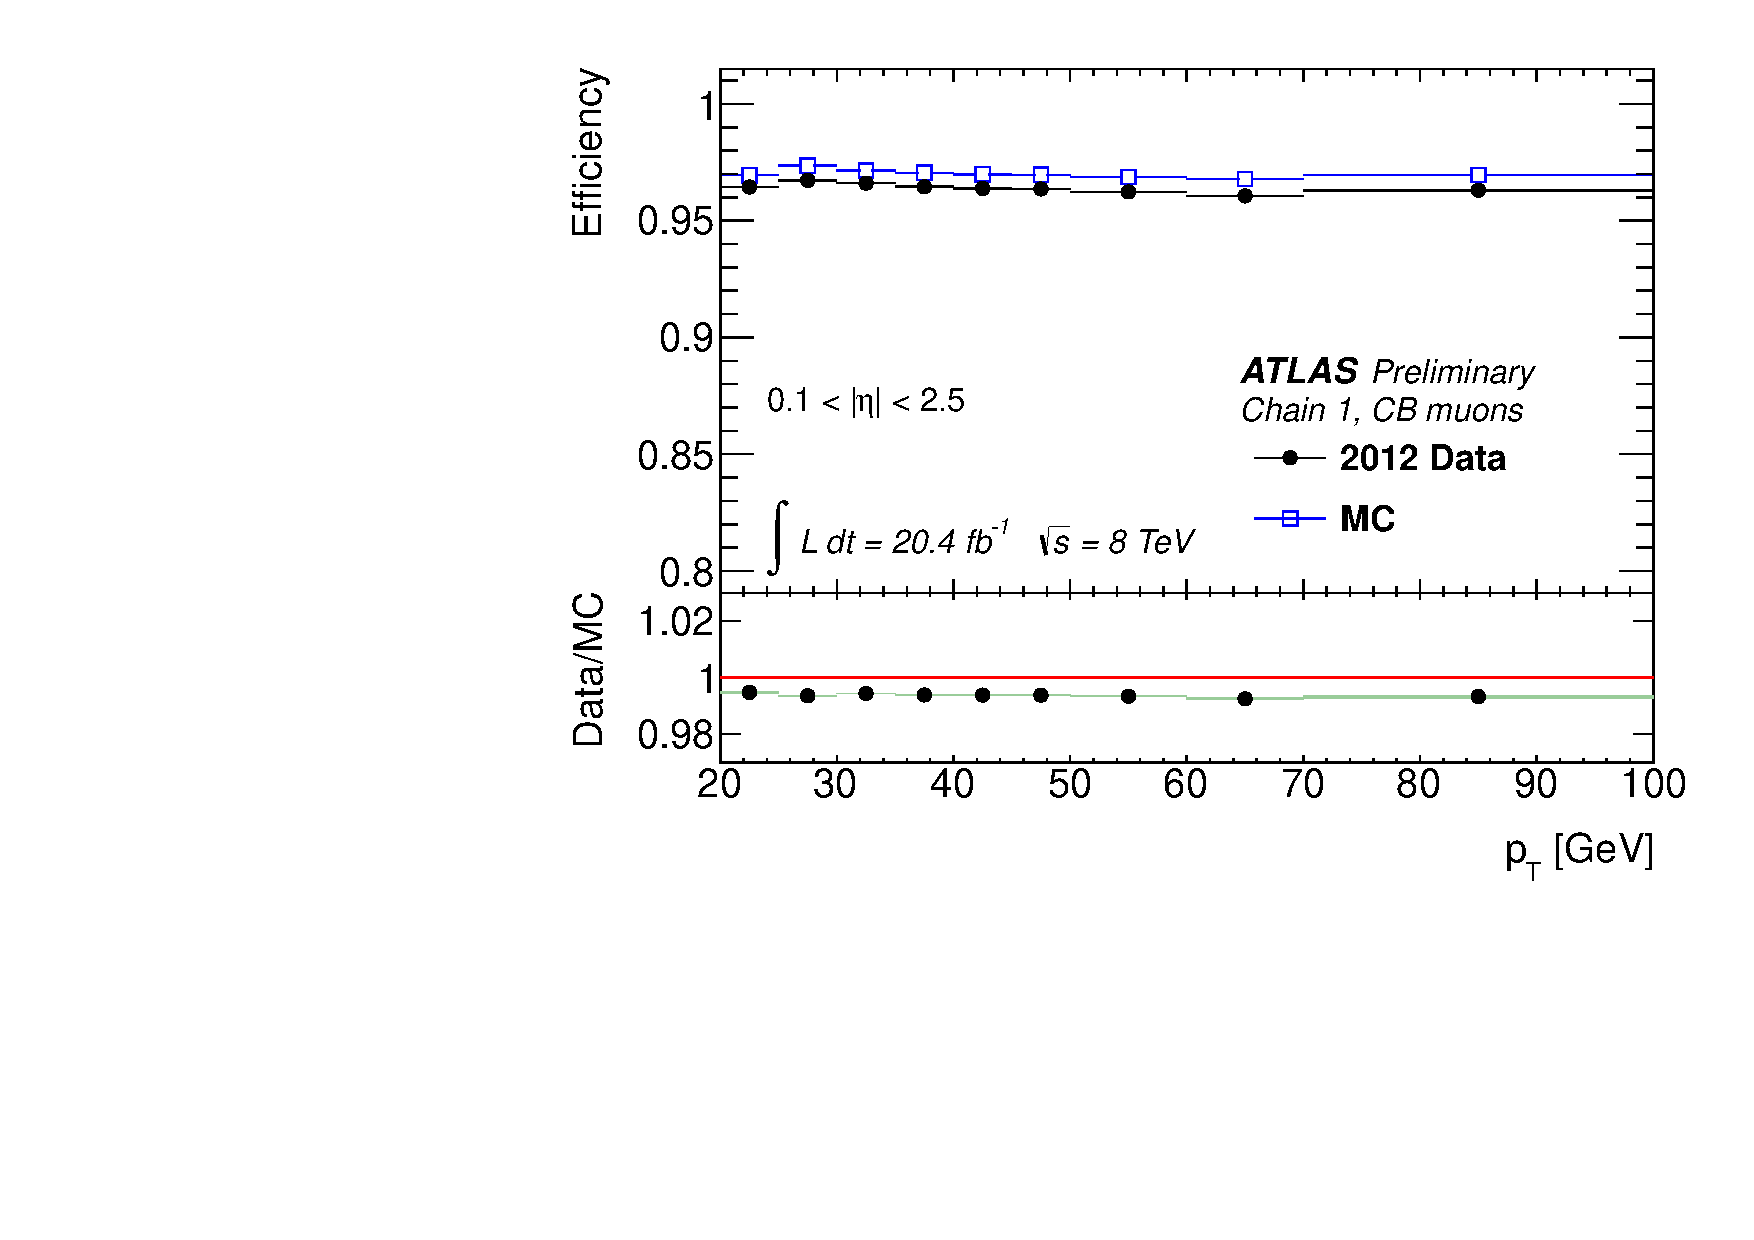
\includegraphics[width=0.495\textwidth]{tex/selection/mu_recoeff_pt}
		\hfill
		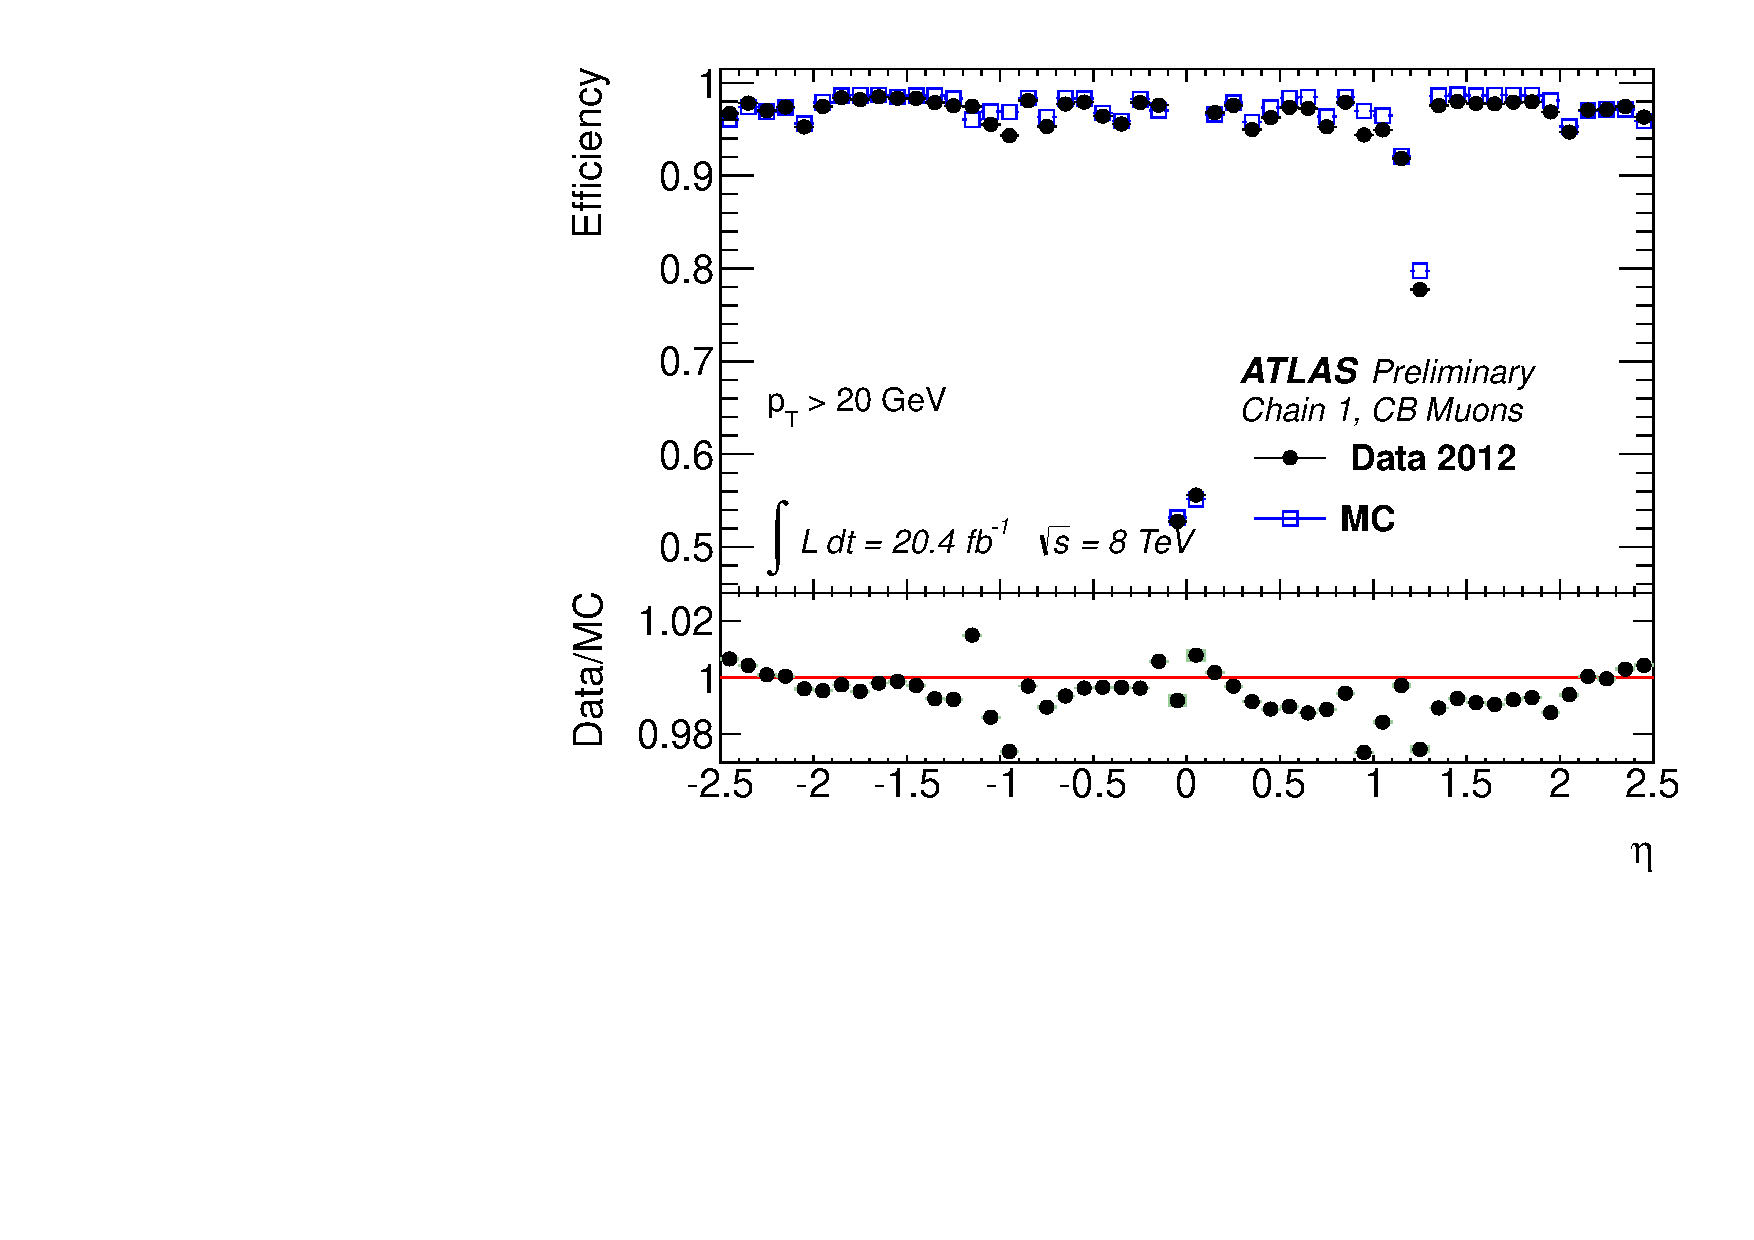
\includegraphics[width=0.495\textwidth]{tex/selection/mu_recoeff_eta}
		\caption{Muon reconstruction efficiency versus \pt (left) and $\eta$ (right), 
		measured using tag-and-probe of \HepProcess{\PZ \HepTo \Pmu\Pmu} data and 
		compared to MC \cite{Muons:2012}. Reductions in efficiency at $\eta \approx 0$ 
		and $\eta \approx 1.2$ are due to partial \ac{MS} coverage (detector services and 
		incomplete installation respectively). `Chain 1' refers to \textit{STACO} 
		reconstruction.}
		\label{fig:objects:mu_recoeff}
	\end{figure}

\end{description}



\subsection{Jets}
\label{sec:objects:jets}

A hadron will pass through the \ac{ID} (leaving hits if charged) before being absorbed by 
the \ac{ECal} and \ac{HCal}. The finite resolution of the calorimeter and the 
large number of overlapping hadronic showers make it impossible to reconstruct individual 
hadrons. For this reason, and more theoretical ones outlined in \Section~\ref{sec:jets}, 
jets are reconstructed from energy deposits. The main challenge in identifying jets from 
the hard scatter is calorimeter noise: electronic and resulting from pile-up.

Jets are selected with $\pt > \unit{25}{\GeV}$ for central jets ($\mods{\eta} < 2.4$) and 
with $\pt > \unit{30}{\GeV}$ for forward jets ($2.4 < \mods{\eta} < 4.5$). However, 
occasionally it is useful to use jets with other \pt thresholds (\eg the central jet 
veto in the VBF search). It shall be clearly stated when this is the case.

\begin{description}
\item[Reconstruction] \hfill \\
	To suppress contributions from calorimeter noise, energy deposits are grouped into 
	topological clusters (\textit{topo-clusters}) \cite{Jets:Calib:2010,Jets:Calib:2011}. 
	First, a seed cell is identified with signal-to-noise ratio $S/N > 4$. Surrounding 
	cells with $S/N > 2$ are iteratively added. Finally, a single iteration of 
	neighbouring cells with no $S/N$ cut are added. When localised maxima exist within a 
	cluster, it may be split. Clearly, the robustness to noise is determined by $N$, 
	which is taken to be the sum in quadrature of the electronic noise and the pile-up 
	noise expected with $\mu = 30$.

	The non-compensating calorimeter design yields different responses to electromagnetic 
	and hadronic showers.\footnote{
		Significant hadronic shower energy is lost through slow neutrons, nuclear 
		excitations and neutrinos.
	}
	Topo-clusters are reconstructed at the EM scale and thus require calibration to the 
	\ac{JES}. An intermediate \textit{local cluster weighting} (LCW) classifies each
	topo-cluster as electromagnetic or hadronic (via energy density and shower depth) 
	and applies an appropriate energy correction.
	
	These topo-clusters are then input to the \antikt jet algorithm with $R = 0.4$ (see 
	\Section~\ref{sec:jets}), making the assumption that the topo-clusters are massless.

\item[Calibration] \hfill \\
	There are four steps to the jet calibration \cite{Jets:Calib:2011}, described below.

	First, the jet direction is adjusted such that it originates from the primary vertex, 
	rather than the centre of the ATLAS coordinate system (a remnant of the jet 
	algorithm).

	Second, energy contributed by pile-up is subtracted \cite{Jets:PileupCorrection:2012}.
	This involves measuring the jet area $A$ (its susceptibility to additional particles 
	with infinitesimal \pt) and the pile-up density $\rho$ of the event. Residual 
	corrections for in-time pile-up (via \npv) and out-of-time pile-up (via $\mu$) are 
	also made. Thus, the correction is
	\begin{equation}
		p_{\text{T}}^{\text{corr}} = \pt - \rho A - \alpha \parenths{\npv - 1} 
		- \beta \parenths{\mu}
	\end{equation}
	and the improved robustness to pile-up that it provides is shown in 
	\Figure~\ref{fig:objects:jet_pu_corr}.

	\begin{figure}
		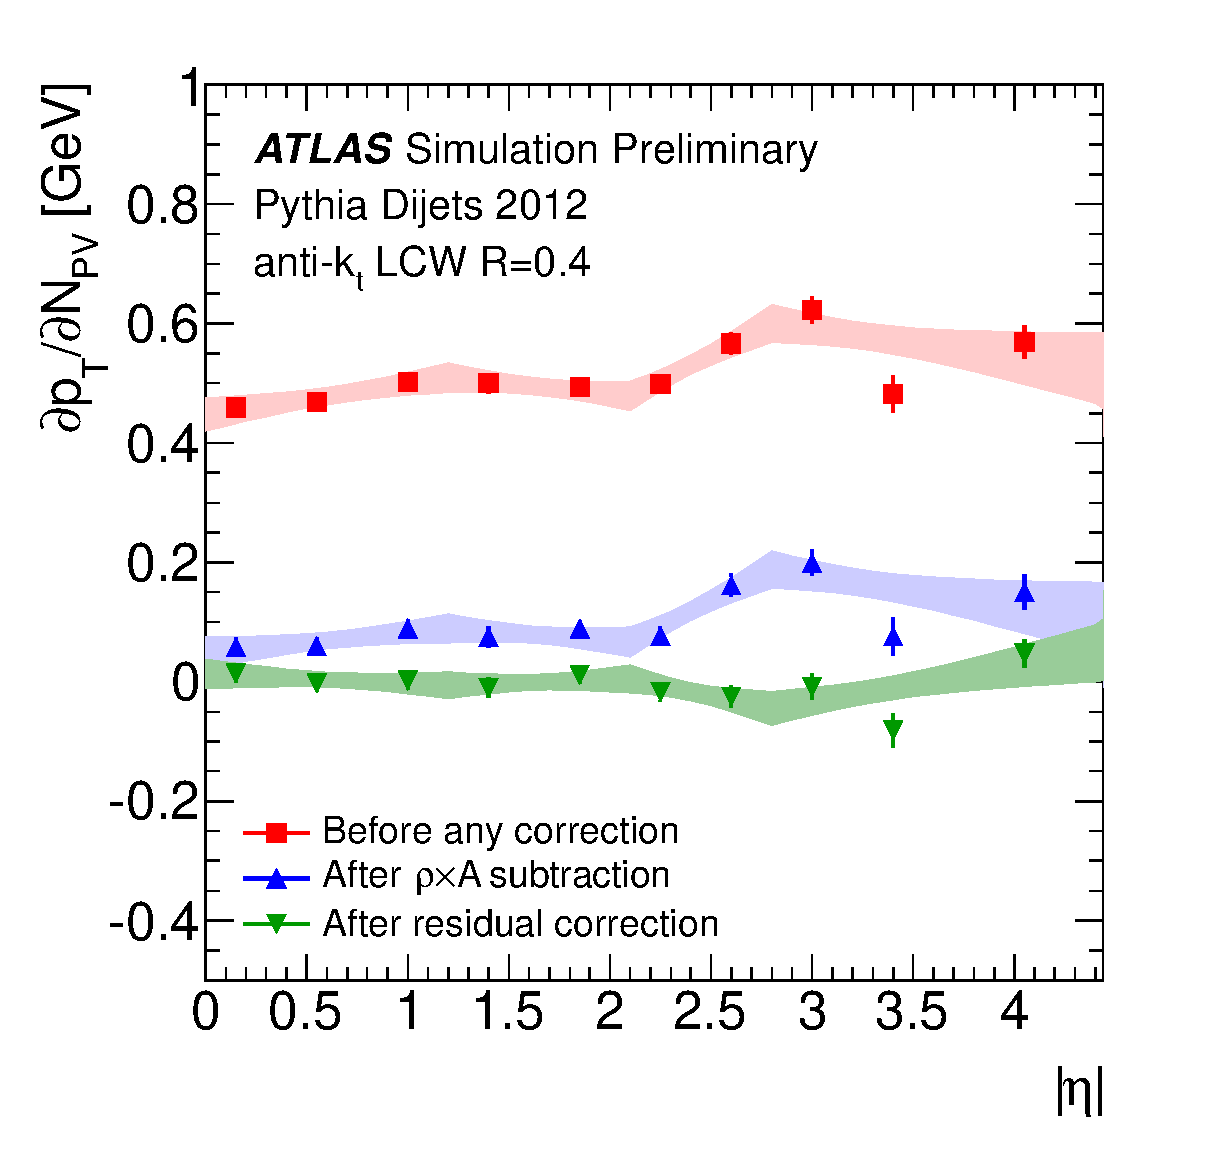
\includegraphics[width=0.495\textwidth]{tex/selection/jet_pu_npv}
		\hfill
		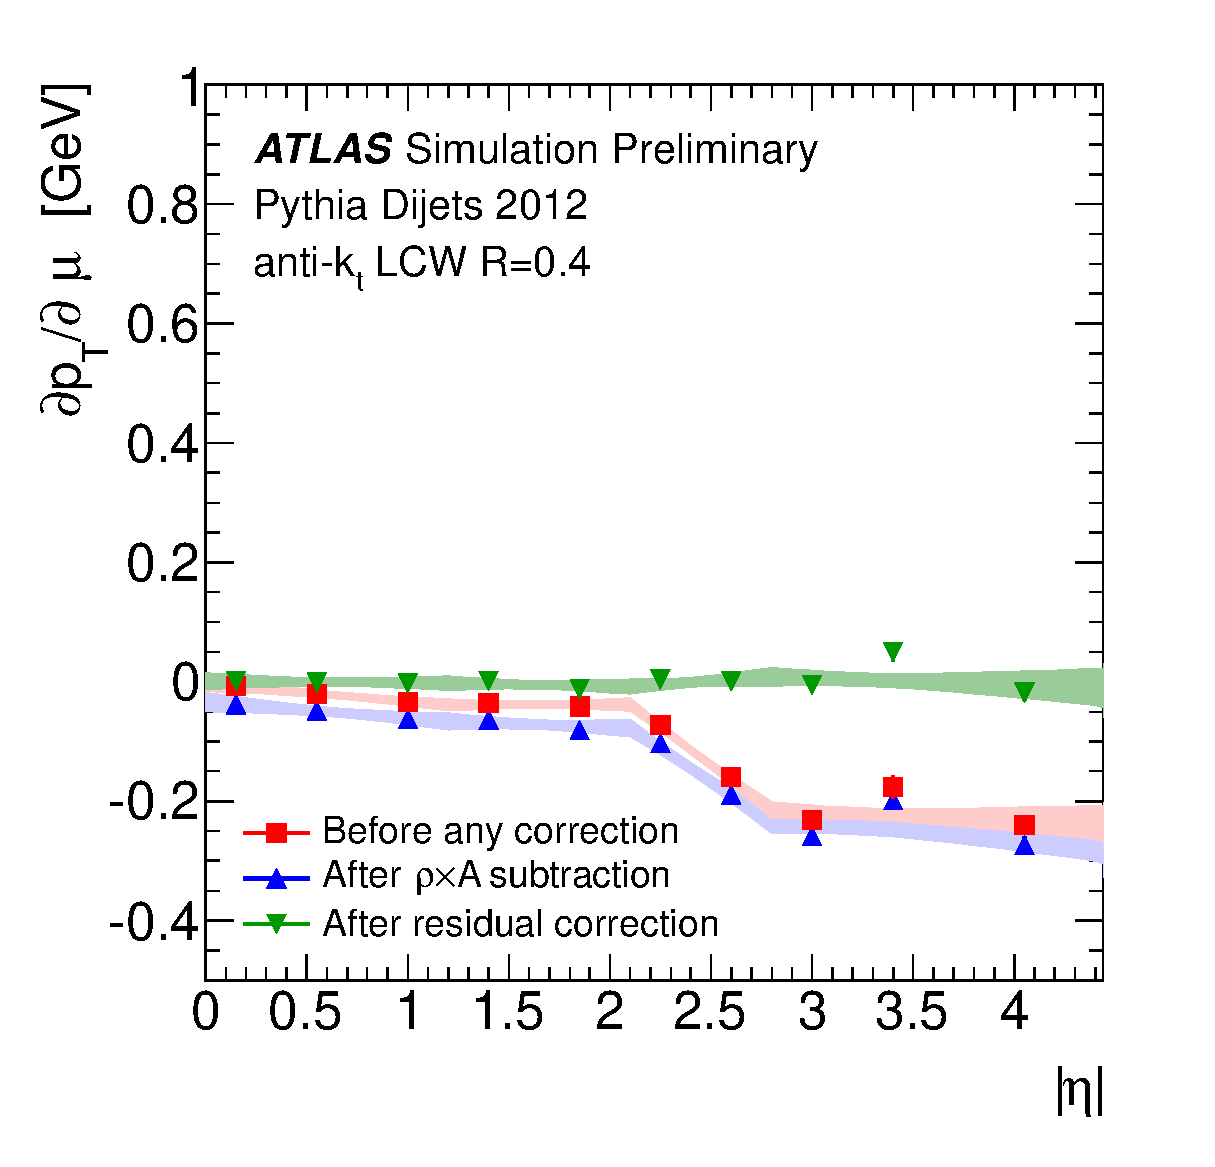
\includegraphics[width=0.495\textwidth]{tex/selection/jet_pu_mu}
		\caption{Dependence of jet \pt on in-time pile-up (left) and out-of-time pile-up 
		(right), versus $\mods{\eta}$ \cite{Jets:PileupCorrection:2012}. The bands show 
		the fits used in the correction.}
		\label{fig:objects:jet_pu_corr}
	\end{figure}

	Third, the energy is calibrated from the LCW scale to the \ac{JES}. The correction is 
	derived from MC by comparing the energy of a reconstructed jet to that of the 
	corresponding hadron-level jet (\ie before detector simulation).

	Finally, a residual \textit{in situ} \ac{JES} calibration corrects for mismodelling, 
	and is applied to jets in data events only. The calibration exploits the \pt 
	balance between a jet and a well-measured reference object, deriving the correction 
	as the double-ratio
	\begin{equation}
		\angles{p_{\text{T}}^{\text{jet}} / p_{\text{T}}^{\text{ref}}}_{\text{\!MC}} 
		\,\, \Big/ 
		\angles{p_{\text{T}}^{\text{jet}} / p_{\text{T}}^{\text{ref}}}_{\text{\!data}} 
		\,\,.
	\end{equation}
	The reference object is chosen to be a \PZ boson (decaying to \epluseminus or 
	\HepProcess{\APmuon\Pmuon}) at low \pt, a photon at medium \pt, or a system of 
	well-calibrated low-\pt jets at high \pt. The contribution of each technique to 
	the correction is shown in \Figure~\ref{fig:objects:jet_insitu}.

	\begin{figure}
		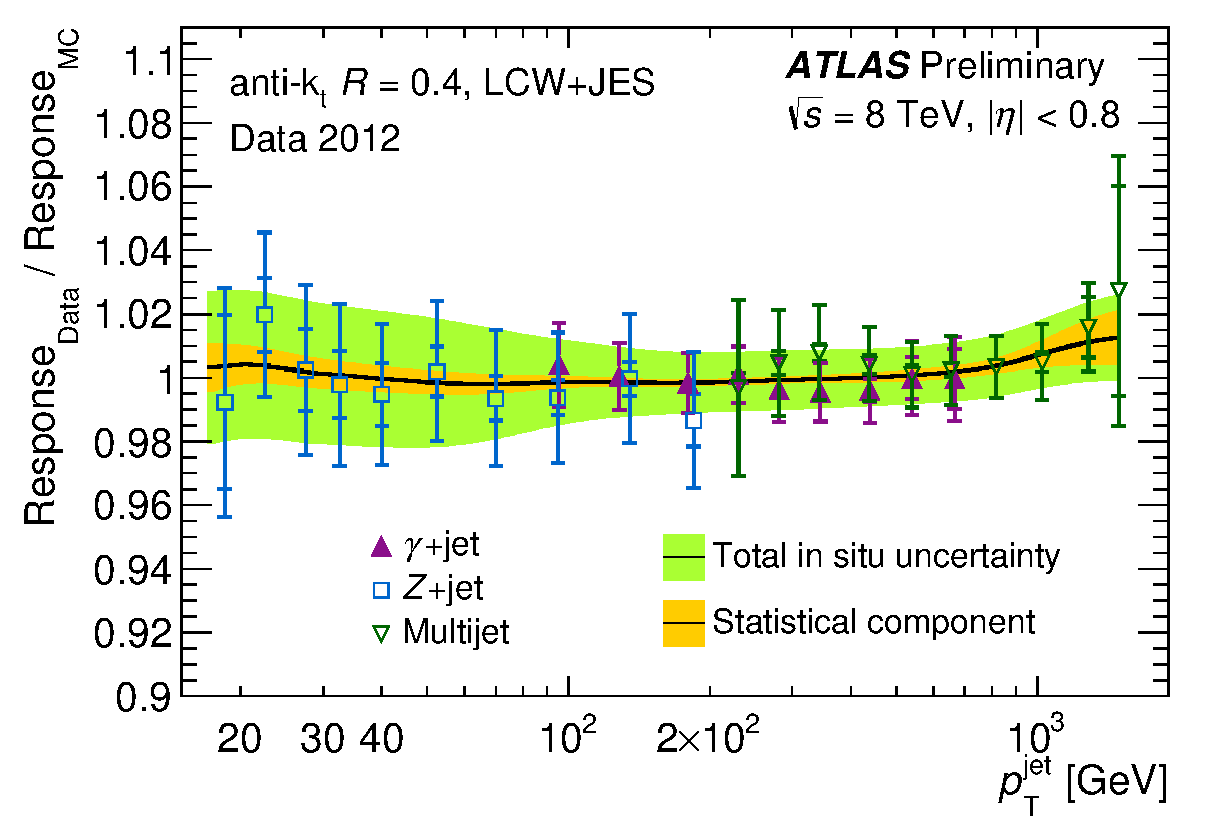
\includegraphics[width=\mediumfigwidth]{tex/selection/jet_insitu_corr}
		\caption{The ratio of the jet response measured in data to the MC prediction 
		versus jet \pt. This is the inverse of the \textit{in situ} JES correction (see 
		text). The results of three \pt balance studies and their combination (black line)
		are shown.}
		\label{fig:objects:jet_insitu}
	\end{figure}

\item[Quality] \hfill \\
	Quality criteria (known as \textit{looser}) reject calorimeter noise based on 
	pulse shapes \cite{Jets:Quality:2011}. The selection is more than 99.8\% efficient 
	for jets with $\pt > \unit{20}{\GeV}$.

\item[Primary vertex association] \hfill \\
	The \textit{jet vertex fraction} (JVF) is defined as the fraction of tracks 
	associated to a jet that originate from the primary vertex ($\mods{z_0 \sin\theta} < 
	\unit{1}{\milli\metre}$), weighted by track \pt \cite{Jets:PileupCorrection:2012}. 
	It is a powerful discriminant against pile-up jets, but is only available for 
	$\mods{\eta} < 2.4$.

	Central jets with $\pt < \unit{50}{\GeV}$ are required to have either 
	$\text{JVF} > 0.5$ or zero associated tracks. The efficiency of this cut is measured 
	\textit{in situ} with \Zjets events.

\end{description}



\subsection{\Pbottom-jets}
\label{sec:objects:bjets}

To aid top background suppression, \textit{\Pbottom-tagging algorithms} exploit the long 
lifetimes of \Pbottom-hadrons to identify jets originating from \Pbottom-quarks. The MV1 
algorithm uses a neural network with inputs of jet \pt, $\eta$ and the weights output 
by three other algorithms \cite{Btag:algorithms}:
\begin{itemize}[noitemsep,nolistsep]
	\item IP3D searches for significant impact parameters of jet tracks, \storeliststyle{}
	\item SV1 searches for secondary vertices associated with \Pbottom-hadron decays,
	\item JetFitter reconstructs the decay chain topology (including the daughter 
	\Pcharm-hadron).
\end{itemize}
An operating point is chosen to tag 85\% of \Pbottom-jets, with a mis-tag rate of 
\about 40\% for \Pcharm-jets, \about 35\% for \Ptau-jets and \about 10\% for light jets
(initiated by \Pup, \Pdown, \Pstrange or \Pgluon). Note that \Pbottom-tagging is only 
available for jets with $\mods{\eta} < 2.5$, since it relies upon tracks.

Modelling \Pbottom-tagging algorithms is very difficult; thus it is imperative to measure 
their efficiency with experimental data. This was done with dileptonic \ttbar events, 
using a combinatorial likelihood method \cite{Btag:llh}. Comparison with MC yields 
efficiency scale factors.



\subsection{Missing transverse momentum}
\label{sec:objects:met}

The near-hermetic detector design enables information of non-interacting particles (\eg 
neutrinos) to be inferred from measurements of interacting particles. Since the initial 
state has no $\bvec{p}_{\text{T}}$, momentum conservation implies that the visible and 
invisible $\bvec{p}_{\text{T}}$ in the final state must balance each other. Thus, the 
negative sum of the visible $\bvec{p}_{\text{T}}$ is known as \textit{missing transverse 
momentum}, and equals the sum of the invisible $\bvec{p}_{\text{T}}$.

Multiple sources of fake momentum imbalance lead to a poor experimental resolution of 
missing transverse momentum. In particular, pile-up has an adverse effect on performance. 
Object mismeasurement can produce a fake imbalance that is highly correlated to the event 
kinematics.

\begin{description}
\item[Calorimeter-based \met] \hfill \\
	One can reconstruct missing transverse momentum with calorimeter energy deposits 
	\cite{MET:2012}. This is denoted \metvec, with magnitude \met, since it is 
	calorimeter-based.

	First, calorimeter cells are associated with and replaced by calibrated high-\pt 
	objects. To avoid double counting, the association is done in a specific order: 
	electrons, photons \cite{Photons:2011}, hadronically decaying \Ptau-leptons 
	\cite{TES:2012}, jets and muons. Note that some object selection criteria are 
	loosened with respect to the preceding descriptions. Importantly, the JVF criterion 
	is removed from jets and their \pt threshold is lowered to \unit{20}{\GeV}. Also, 
	segment-tagged muons are used in addition to combined muons.

	The low-\pt component is reconstructed using topo-clusters of the remaining deposits 
	(for noise suppression), which are calibrated to the LCW scale (see 
	\Section~\ref{sec:objects:jets}). This is improved further by including unassociated 
	tracks with \unit{$\pt > 400$}{\MeV}.

	Thus, the missing transverse momentum is defined with the following components
	\begin{equation}
		\metvec = - \braces{ 
		\sum\limits_{\Pe} \ptvec + 
		\sum\limits_{\Pmu} \ptvec + 
		\sum\limits_{\Ptau} \ptvec + 
		\sum\limits_{\Pphoton} \ptvec + 
		\sum\limits_{\text{jets}} \ptvec + 
		\sum\limits_{\text{soft}} \ptvec
		} \,.
	\end{equation}
	Unfortunately, \met is highly susceptible to pile-up because the starting points are 
	calorimeter cells, which are not easily associated to the primary vertex. Performance 
	can be improved by a JVF cut on jets and implementing a similar idea on the soft 
	contributions. However, for the \HWWlvlv search, it was found that the best pile-up 
	performance was achieved by using tracks as the starting points.

\item[Track-based \trackmet] \hfill \\
	One can alternatively reconstruct missing transverse momentum with \ac{ID} tracks. 
	This is denoted \trackmetvec, with magnitude \trackmet, since it is track-based.

	Tracks with \unit{$\pt > 500$}{\MeV} are selected if they have sufficiently small 
	impact parameters with respect to the primary vertex 
	(\unit{$\mods{d_0} < 1.5$}{\milli\metre} and 
	\unit{$\mods{z_0\sin\theta} < 1.5$}{\milli\metre}). Quality criteria require 
	$n_{\text{pixel}}^{\text{hit}} \geq 1$ and $n_{\text{SCT}}^{\text{hit}} \geq 6$. 
	Additional tracks may be used if they are associated with a lepton with 
	$\unit{$\mods{z_0\sin\theta} < 1.0$}{\milli\metre}$ (the electron identification 
	criteria are loosened to medium \cf \Section~\ref{sec:objects:electrons}, and the 
	muon \pt threshold is lowered to \unit{6}{\GeV} \cf \Section~\ref{sec:objects:muons}).

	Occasionally, tracks are poorly reconstructed, which can have a significant impact 
	upon \trackmet. Therefore, tracks with \unit{$\pt > 100$}{\GeV} that are not 
	associated to any physics object are removed from the selection. Similarly, a track 
	within $\Delta R < 0.4$ of a jet with \unit{$\pt > 10$}{\GeV} is removed if 
	$p_{\text{T}}^{\text{track}} > 1.4 \, p_{\text{T}}^{\text{jet}}$.

	Bremsstrahlung from an electron can convert to \epluseminus pairs, resulting in 
	additional tracks. For this reason, tracks within a cone of $\Delta R < 0.05$ of a 
	reconstructed electron are collectively replaced with the calibrated electron \pt.
	Muon \ac{ID} tracks are also replaced by the \pt of the reconstructed muon.

	Thus, the missing transverse momentum is defined with the following components
	\begin{equation}
		\trackmetvec = - \braces{ 
		\sum\limits_{\Pe} \ptvec + 
		\sum\limits_{\Pmu} \ptvec + 
		\!\!\!\! \sum\limits_{\text{unassoc.}} \!\!\!\! \ptvec
		} \,.
	\end{equation}
	\trackmet is very resilient to pile-up. However, its inability to include neutral 
	hadrons significantly degrades the resolution.

\item[Jet-corrected track-based \corrtrackmet] \hfill \\
	It is possible to correct \trackmet for neutral hadrons with calorimeter information. 
	Tracks within a cone of $\Delta R < 0.4$ of a jet are collectively replaced by the 
	calibrated jet \pt.

	Thus, the missing transverse momentum is defined with the following components
	\begin{equation}
		\corrtrackmetvec = - \braces{ 
		\sum\limits_{\Pe} \ptvec + 
		\sum\limits_{\Pmu} \ptvec + 
		\sum\limits_{\text{jets}} \ptvec + 
		\!\!\!\! \sum\limits_{\text{unassoc.}} \!\!\!\! \ptvec
		} \,.
	\end{equation}
	This has the best resolution, but the use of calorimeter information does introduce 
	some pile-up dependence.

\item[Relative missing transverse momentum] \hfill \\
	The effect of object mismeasurement upon missing transverse momentum can be reduced 
	by considering the component transverse to the nearest reconstructed object. Thus, 
	the relative \met is defined to be
	\begin{equation}
		\metrel = 
		\begin{cases}
			\met\sin\parenths{\Delta\phi} & \text{if~} \Delta\phi < \pi/2 \\
			\met & \text{otherwise}
		\end{cases}
	\end{equation}
	where $\Delta\phi$ is the angle between \metvec and the nearest electron, muon or jet.
	Similar definitions exist for \trackmetrel and \corrtrackmetrel.

\end{description}



\subsection{Object overlap removal}
\label{sec:objects:overlap}

In order to avoid double-counting calorimeter deposits and tracks as multiple physics 
objects, overlapping objects are removed according to the following rules:

\begin{listliketab}
	\begin{tabular}{Ll@{\hskip 0.3in}l}
		\textbullet & $\Delta R \parenths{\Pe,\Pmu} < 0.1$ & remove electron \\
		\textbullet & $\Delta R \parenths{\Pe,\Pe}  < 0.1$ & remove electron with lower \pt \\
		\textbullet & $\Delta R \parenths{\Pe,j}    < 0.3$ & remove jet \\
		\textbullet & $\Delta R \parenths{\Pmu,j}   < 0.3$ & remove muon \\
	\end{tabular}
\end{listliketab}

